\lstdefinestyle{ubuntu}
{
    backgroundcolor=\color{black},
    basicstyle=\scriptsize\color{green}%\ttfamily
}
\chapter{Interfacing da Vinci with ROS}\label{app:ros}
This appendix ought to give concrete knowlegde to utilize the \gls{ros} environment wrt. the \gls{daVinci} surgery robot at Aalborg University as it comprises an immense load of files, packages and various GUI interfaces. The \gls{ros} environment is currently only developed for Ubuntu. The content of this appendix is accordingly assuming Ubuntu as operating system and assumes additionally basic knowledge in Unix, that a ROS workspace is created ({\color{blue}{\textit{http://wiki.ros.org/catkin/Tutorials/create\_a\_workspace}}}) and that all the code located at the "Robotic Surgery Group - Aalborg University" has been copied/cloned to the root of the workspace ({\color{blue}{\textit{https://github.com/AalborgUniversity-RoboticSurgeryGroup/}}}).

The original environment (clean configuration) can be cloned with the following git terminal commands:\vspace{0.1cm}

\hspace{0cm} \texttt{\$ git clone https://github.com/AalborgUniversity-RoboticSurgeryGroup/davinci\_description}

\hspace{0cm} \texttt{\$ git clone https://github.com/AalborgUniversity-RoboticSurgeryGroup/davinci\_driver}

\hspace{0cm} \texttt{\$ git clone https://github.com/AalborgUniversity-RoboticSurgeryGroup/davinci\_moveit\_config}\vspace{0.1cm}

Each command copies a so called \gls{ros} package which initially are created by the \texttt{catkin\_create\_pkg} command. A "package" is simply the name convention for a chunk of software. The name and file structure of a package should follow a certain standard, i.e. the \gls{rep}. This ought to make it easier to share and reuse code. The code developed in this thesis obeys to some extend the \gls{rep}s but exceptions may occur. 

The development branch, i.e. the result of the work undertaken in this project, can be cloned as:

\hspace{0cm} \texttt{\$ git clone <URL> ---branch develop} \ \ \ {\color{RoyalBlue}{\textit{\# Clone all three packages}}}

After the workspace is created (call it \texttt{daVinci\_ws}) and the packages are cloned, the overall code structure should look like the tree structure found below:

\vspace{0.5cm}

\begin{tikzpicture}[scale=1]
\Tree [.\color{blue}{\texttt{daVinci\_ws}}
  [.\color{blue}{\texttt{build}} \text{make files etc.} ]  [.\color{blue}{\texttt{devel}} lib/setup ]  
     [.\color{blue}{\texttt{src}} {\color{white}{m}}$\underset{\text{input to the CMake build system}}{\text{\color{ForestGreen}{\texttt{CMakeLists.txt}}}}${\color{white}{m}} [.\hspace{0.2cm}\text{package $1$}\hspace{0.2cm} $\cdots$ $\cdots$ ]
     [.\hspace{0.2cm}\text{package 2}\hspace{0.2cm} $\cdots$ $\cdots$ ] \hspace{0.2cm}$\cdots$\hspace{0.2cm}  [.\hspace{0.2cm}\text{package $n$}\hspace{0.2cm} $\cdots$ $\cdots$  ]   ] 
  ]
\end{tikzpicture}
  
\vspace{0.2cm}

The package where most of the development in this thesis takes place is in the \texttt{davinci\_moveit\_config} package located in the \texttt{src} folder. To give some idea of the content and how the code is structured, the directory tree on the following page is provided. It shows merely the "interesting files" seen from a developers point of view. In reality, additionally files are present. 

\begin{comment}
\hspace{-1.5cm}
 \Tree [.\color{blue}{\texttt{daVinci\_ws}} 
 %[.\scriptsize  \texttt{build/} \text{all make-files}\\\text{(auto-generated}) ] 
  [.\scriptsize  \texttt{src/} 
  %\scriptsize  \color{green}{\texttt{CMakeLists.txt}} 
  \scriptsize \texttt{davinci\_}\\\scriptsize \texttt{description/}	 
[.\scriptsize \texttt{davinci\_}\\\scriptsize \texttt{moveit\_config/} \scriptsize  \color{green}{\texttt{CMakeLists.txt}} [.\texttt{src} \scriptsize \texttt{MoveGroupInterface.cpp}\\\text{(main C++ interface)} ]  \scriptsize  \texttt{config}  \texttt{launch}  \color{green}{\texttt{package.xml}} ]   
  \scriptsize \texttt{davinci\_}\\\scriptsize \texttt{driver/} ]  
  %[.\scriptsize  \texttt{devel/} \text{setup files +}\\\text{libraries etc.} ] 
  ] 
\end{comment}
\newpage

%[.\texttt{davinci\_moveit\_config} \texttt{config} \texttt{launch} ] \texttt{davinci\_description} \texttt{davinci\_driver} [.VP [.V is ] \qroof{a simple tree}.NP ] ]

\renewcommand*\DTstylecomment{\rmfamily\color{gray}\textsc}
\renewcommand*\DTstyle{\ttfamily\textcolor{blue}}

\begin{figure}[H]
% to make comment:
% .4 davinci\_moveit\_config\DTcomment{Guillaume}.
\dirtree{%
.1 /...
.2 davinci\_ws. %\DTcomment{workspace folder, created by mkdir}.
.3 build. %\DTcomment{generated by catkin\_init\_workspace}.
%.4 \color{gray}{..}.
.4 \color{gray}{... all make-files}. %\DTcomment{generated by catkin\_init\_workspace}.
.3 devel. %\DTcomment{generated by catkin\_init\_workspace}.
%.4 \color{gray}{..}.
.4 \color{gray}{... all libraries and setup files}. %\DTcomment{generated by catkin\_init\_workspace}.
.3 src.
.4 \color{ForestGreen}{CMakeLists.txt}.
.4 davinci\_description. %\DTcomment{\underline{Package:} Physical sizes and rotation matrices}.
.5 \color{ForestGreen}{CMakeLists.txt}.
.5 config.
.6 \color{ForestGreen}{davinci.rviz}.
.5 launch.
.6 \color{ForestGreen}{demo.launch}.
.6 \color{ForestGreen}{visualize\_in\_rviz.launch}.
.5 meshes.
.6 \color{gray}{... all .stl files (used for the 3D model in rviz)}.
.5 \color{ForestGreen}{package.xml}.
.5 robots.
.6 \color{ForestGreen}{remote\_center\_manipulator.xacro}\hspace{0.5cm}\color{gray}{\# rotation matrices for the hand}.
.6 \color{ForestGreen}{davinci.xacro}\hspace{0.5cm}\color{gray}{\# assembles all xml macros}.
.6 \color{ForestGreen}{p4\_arm.xacro}\hspace{0.5cm}\color{gray}{\# rotation matrices for the arm}.
.6 instruments.
.7 \color{ForestGreen}{needle\_driver.xacro}\hspace{0.5cm}\color{gray}{\# rotation matrices for instrument}.
.4 davinci\_driver. %\DTcomment{\underline{Package:} Interface with the physical robot}.
.5 \color{ForestGreen}{CMakeLists.txt}.
.5 \color{ForestGreen}{dstp.json}.
.5 launch.
.5 src.  
.6 \color{ForestGreen}{davinci\_driver.cpp}\hspace{0.5cm}\color{gray}{\# ...}.
.6 \color{ForestGreen}{ros\_driver.cpp}\hspace{0.5cm}\color{gray}{\# ...}.
.6 \color{ForestGreen}{sbrio\_driver.cpp}\hspace{0.5cm}\color{gray}{\# ...}.
.5 srv.
.6 \color{gray}{... various hard-coded names}.
.5 config.
.6 \color{ForestGreen}{davinci\_ip\_adresses.yaml}\hspace{0.5cm}\color{gray}{\# set IP for RIO primary/secondary board}.
.6 \color{ForestGreen}{p4\_hand\_controller.yaml}\hspace{0.5cm}\color{gray}{\# specify each controllable joint}.
.5 include.
.6 \color{gray}{... header files for davinci\_driver.cpp and sbrio\_driver.cpp}.
.5 libsjon.
.6 \color{gray}{... various libraries}.
.4 davinci\_moveit\_config. %\DTcomment{\underline{Package:} Trajectory planning}.
.5 \color{ForestGreen}{CMakeLists.txt}.
.5 config.
.6 \color{ForestGreen}{controllers.yaml}\hspace{0.5cm}\color{gray}{\# specifies each controllable joint}.
.6 \color{ForestGreen}{davinci.srdf}\hspace{0.5cm}\color{gray}{\# collision states, group states and group specification}.
.6 \color{ForestGreen}{fake\_controllers.yaml}\hspace{0.5cm}\color{gray}{\# simulation controller specification}.
.6 \color{ForestGreen}{joint\_limits.yaml}\hspace{0.5cm}\color{gray}{\# Acceleration, velocity and position limits}.
.6 \color{ForestGreen}{kinematics.yaml}\hspace{0.5cm}\color{gray}{\# Kinematic solver specification}.
.6 \color{ForestGreen}{ompl\_planning.yaml}\hspace{0.5cm}\color{gray}{\# path planning specification}. 	
.5 launch.
.6 \color{ForestGreen}{davinci\_moveit\_controller\_manager.launch.xml}\hspace{0.5cm}\color{gray}{}.
.6 \color{ForestGreen}{move\_group.launch}\hspace{0.5cm}\color{gray}{\# launch all essential drivers }.
.6 \color{ForestGreen}{setup\_assistant.launch}\hspace{0.5cm}\color{gray}{\# launch to generate essential moveit files}.
.6 \color{gray}{... + a number of other launch files controlled by the setup assistant}.
.5 \color{ForestGreen}{package.xml}\hspace{0.5cm}\color{gray}{\# specification of moveit dependencies}.
.5 src.
.6 \color{ForestGreen}{MoveGroupInterface.cpp}\hspace{0.5cm}\color{gray}{\# main C++ interface}.
}
%\caption{Code structure in the ROS environment}
\end{figure}

%Be very sure to clone all three packages.
\subsubsection*{Setup of Low Level Control}
Before the communication between ROS and da Vinci may be considered, all low level PID controllers must run correctly and the RIO configuration must be performed. 

From the \texttt{aau86730} computer, launch the \texttt{p4\_primary\_Control} icon located on the desktop and connect \texttt{RT Single Board RIO (172.26.12.32)} by right clicking the icon and press connect. Subsequently, navigate to \texttt{p4\_prim\_control\_FPGA\_multichannel\_7\_FLOAT\_SPI\_5.vi} and open it. This launch a GUI comprising access to the seven low level controllers which are activated from the arrow in the upper left corner. The controller gains, setpoints, maximum step size and various calibration options are easily accessible from this GUI, though it should not be necessary to modify any of those. 

Be sure that the gearing factors are specified as follows:
\begin{table}[H]
\begin{tabularx}{\textwidth}{X X X X X X X}
\rowcolor{HeaderBlue} 
\scriptsize \textbf{Intrument Jaw Left} &\scriptsize  \textbf{Intrument Jaw Right} &\scriptsize  \textbf{Intrument Jaw Pitch} &\scriptsize  \textbf{Instrument Pitch} &\scriptsize  \textbf{Instrument Roll} & \scriptsize   \textbf{Hand Pitch} &  \scriptsize\textbf{Hand Roll}\\
12 & 12 & 12.4 & 7.5 & 1340 & 200 & 200\\
\end{tabularx}
	\caption{Measured gearing factors. Gearing factors are measured such that $\pi$/4 from \gls{ros} corresponds to 45 degrees on the real robot.}
\label{tab:gearing}
\end{table}
To allow the ROS environment access to the full range of setpoints, launch \texttt{p4-control\_prim-main4.vi} and activate this GUI in a similar manner. This GUI acts merely as interface and offers no user options as such. All necessary setup before initiating ROS is at this point in time performed.
\subsubsection*{ROS}
To communicate with da Vinci, it is important to execute a few commands in the correct order from the \texttt{surgery-srv.lab.es.aau.dk} computer. It is recommended to work directly on the server in the lab (it provides additional GUI applications such as rviz), but connection to a private laptop can be established through \texttt{ssh}:

%\begin{lstlisting}[style=ubuntu]
\hspace{1cm} \texttt{\$ ssh <user>@surgery-srv.lab.es.aau.dk}
%\end{lstlisting}

Every time a new terminal is commenced it is important to source the bash file from the workspace, i.e.:

\hspace{1cm} \texttt{\$ source devel/setup.bash}

It is first of all important to collect all \gls{node}s such that they are able to communicate with each other. The following list of commands must be executed from the root of the workspace. Open a terminal an run:

\hspace{1cm} \textbf{1.} \ \ \ \texttt{\$ roscore} \ \ \ {\color{RoyalBlue}{\textit{\# Leave this running in the terminal}}}

Now, to secure the TCP/IP connection between ROS and the RIO board (Rx \& Tx of setpoints), launch the driver from a new terminal:

\hspace{1cm} \textbf{2.} \ \ \  \texttt{\$ roslaunch davinci\_driver davinci\_driver.launch} \ \ \ {\color{RoyalBlue}{\textit{\# Leave this running}}} 

To allow trajectory planning, link the OMPL (Open Motion Planning Library) to the system by running: 

\hspace{1cm} \textbf{3.a} \ \ \  \texttt{\$ roslaunch davinci\_moveit\_config move\_group.launch} \ \ \ {\color{RoyalBlue}{\textit{\# Leave this running}}} 

If a 3D GUI interface is desired, open a new terminal and launch:

\hspace{1cm} \textbf{3.b} \ \ \  \texttt{\$ roslaunch davinci\_bringup visualization.launch} \ \ \ {\color{RoyalBlue}{\textit{\# This opens rviz}}} 

Press the "add" button in \texttt{rviz} and add the "MotionPlanning" option to the panel where start and goal state can be specified. Hereafter, plan and execute the specified goal. This cause the arm of da Vinci to reach out for the specified goal state consisting of five joint angles.

\subsubsection*{Useful and Regularly used ROS Commands}
To build the entire environment, navigate to the root of the workspace and type:

\hspace{1cm} \textbf{$\bullet$} \ \ \  \texttt{\$ catkin\_make}% \ \ \ {\color{RoyalBlue}{\textit{\# read various state information from terminal output}}} 

The current joint position is per default broadcasted to the topic \texttt{joint\_states}. To subscribe to this topic, open a terminal and type:

\hspace{1cm} \textbf{$\bullet$} \ \ \  \texttt{\$ rostopic echo joint\_states} \ \ \ {\color{RoyalBlue}{\textit{\# read various state information from terminal output}}} 

Obtain a list of the used kinematic solvers, open a terminal and type:

\hspace{1cm} \textbf{$\bullet$} \ \ \  \texttt{\$ rosparam list | grep kinematics} \ \ \ {\color{RoyalBlue}{\textit{\# read solvers from terminal}}} 

view to all active topics:

\hspace{1cm} \textbf{$\bullet$} \ \ \  \texttt{\$ rostopic list} \ \ \ {\color{RoyalBlue}{\textit{\# read topics from terminal}}} 

To create a \gls{urdf} file from the present xacro files, type the below command from the root of the workspace:

\hspace{1cm} \textbf{$\bullet$} \ \ \  \texttt{\$ rosrun xacro xacro.py src/davinci\_description/robots/davinci.xacro > <name>.URDF} %\ \ \ {\color{RoyalBlue}{\textit{\# URDF is created}}} 
%
\subsection*{Setup Assistant}
To run the setup assistant, open a terminal, navigate to the root of the workspace and type:

\hspace{1cm} \textbf{$\bullet$} \ \ \  \texttt{\$ roslaunch davinci\_moveit\_config setup\_assistant.launch} \ \ \ {\color{RoyalBlue}{\textit{\# GUI is launched}}} 

Files that needs to be created/modified manually when the setup assistant is launched:
\begin{itemize}
	\item \texttt{src/davinci\_moveit\_config/launch/davinci\_moveit\_controller\_manager.launch}
	\item \texttt{src/davinci\_moveit\_config/config/controllers.yaml}
\end{itemize}

\subsection*{Useful Debugging Commands}
To check which files are recently modified, open a terminal and run:

\hspace{1cm} \textbf{$\bullet$} \ \ \  \texttt{\$ find . -type f -exec ls -lt $\backslash$\{$\backslash$\} $\backslash$+ | head} 

This is fairly useful as, for example, the setup-assistant overwrites a number of files. 

{\color{white}{\gls{yaml}}}{\color{white}{\gls{xacro}}}

